%%%%(c)
%%%%(c)  This file is a portion of the source for the textbook
%%%%(c)
%%%%(c)    Abstract Algebra: Theory and Applications
%%%%(c)    Copyright 1997 by Thomas W. Judson
%%%%(c)
%%%%(c)  See the file COPYING.txt for copying conditions
%%%%(c)
%%%%(c)
\chap{Fields}{fields}

It is natural to ask whether or not some field $F$ is contained in a
larger field.  We think of the rational numbers, which reside inside
the real numbers, while in turn, the real numbers live inside the
complex numbers.  We can also study the fields between ${\mathbb Q}$ and
${\mathbb R}$ and inquire as to the nature of these fields.

 
More specifically if we are given a field $F$ and a polynomial $p(x)
\in F[x]$, we can ask whether or not we can find a field $E$
containing $F$ such that $p(x)$ factors into linear factors over
$E[x]$.  For example, if we consider the polynomial  
\[
p(x) =x^4 -5 x^2 + 6
\]
in ${\mathbb Q}[x]$,  then $p(x)$ factors as $(x^2 - 2)(x^2 - 3)$.
However, both of these factors are irreducible in ${\mathbb Q}[x]$.  If
we wish to find a zero of $p(x)$, we must go to a larger field.
Certainly the field of real numbers will work, since
\[
p(x) = (x - \sqrt{2} ) (x + \sqrt{2} )( x - \sqrt{3})(x + \sqrt{3}).
\]
It is possible to find a smaller field in which $p(x)$ has a zero,
namely 
\[
{\mathbb Q }( \sqrt{2} ) = \{ a + b \sqrt{2} : a, b \in {\mathbb Q} \}. 
\]
We wish to be able to compute and study such fields for arbitrary 
polynomials over a field $F$.  


\section{Extension Fields}

A field $E$ is an {\bfi extension
field\/}\index{Extension!field}\index{Field!extension} of a field $F$
if $F$ is a subfield of $E$. The field $F$ is called the {\bfi base 
field}\index{Field!base}.  We write $F \subset E$.

\begin{example}{field_Q_sqrt2}
For example, let 
\[
F = {\mathbb Q}( \sqrt{2}\,) = \{ a + b \sqrt{2} : a, b \in {\mathbb Q} \}
\]
and
let
$E =  {\mathbb Q }( \sqrt{2} +  \sqrt{3}\,)$ be the smallest field
containing both ${\mathbb Q}$ and $\sqrt{2} + \sqrt{3}$. Both $E$ and $F$
are extension fields of the rational numbers. We claim that $E$ is an
extension field of $F$. To see this, we need only show that $\sqrt{2}$
is in $E$. Since $\sqrt{2} + \sqrt{3}$ is in $E$, $1 / (\sqrt{2} +
\sqrt{3}\,) = \sqrt{3} - \sqrt{2}$ must also be in $E$. Taking linear
combinations of $\sqrt{2} + \sqrt{3}$ and $\sqrt{3} - \sqrt{2}$, we
find that $\sqrt{2}$ and $\sqrt{3}$ must both be in $E$.
\end{example}


\begin{example}{finite_field4}
Let $p(x) = x^2 + x + 1 \in {\mathbb Z}_2[x]$. Since neither 0 nor 1 is a
root of this polynomial, we know that $p(x)$ is irreducible over
${\mathbb Z}_2$. We will construct a field extension of ${\mathbb Z}_2$
containing an element $\alpha$ such that $p(\alpha) = 0$. By
Theorem~\ref{poly:max_ideal_theorem}, the ideal $\langle p(x) \rangle$ generated by $p(x)$
is maximal; hence, ${\mathbb Z}_2[x] / \langle p(x) \rangle$ is a field. 
Let $f(x) + \langle p(x) \rangle$ be an arbitrary element of
${\mathbb Z}_2[x] / \langle p(x) \rangle$. By the division algorithm,   
\[
f(x) = (x^2 + x + 1) q(x) + r(x),
\]
where the degree of $r(x)$ is less than the degree of $x^2 + x + 1$.
Therefore, 
\[
f(x) + \langle x^2 + x + 1 \rangle = r(x) + \langle x^2 + x + 1
\rangle. 
\]
The only possibilities for $r(x)$ are then $0$, $1$, $x$, and $1+x$.
Consequently, $E = {\mathbb Z}_2[x] / \langle x^2 + x + 1 \rangle$ is a field
with four elements and must be a field extension of ${\mathbb Z}_2$,
containing a zero $\alpha$ of $p(x)$. The field ${\mathbb Z}_2(  \alpha)$
consists of elements  
\begin{align*}
0 + 0 \alpha & = 0 \\
1 + 0 \alpha & = 1 \\
0 + 1 \alpha & = \alpha \\
1 + 1 \alpha & = 1 + \alpha.
\end{align*}
Notice that ${\alpha}^2 + {\alpha} + 1 = 0$; hence, if we compute $(1
+ \alpha)^2$,  
\[
(1 + \alpha)(1 + \alpha)= 1 + \alpha + \alpha + (\alpha)^2 = \alpha. 
\]
Other calculations are accomplished in a similar manner.  We summarize
these computations in the following tables, which tell us how to add
and multiply elements in $E$.
\begin{center}
\begin{tabular}{c|cccc}
+            & 0            & 1            & $\alpha$     & $1 + \alpha$ \\
\hline
0            & 0            & 1            & $\alpha$     & $1 + \alpha$ \\
1            & 1            & 0            & $1 + \alpha$ & $\alpha$ \\
$\alpha$     & $\alpha$     & $1 + \alpha$ & 0            & 1 \\
$1 + \alpha$ & $1 + \alpha$ & $\alpha$     & 1            & 0  
\end{tabular}
\end{center}
\medskip
\begin{center}
\begin{tabular}{c|cccc}
$\cdot$      & 0 & 1             & $\alpha$     & $1 + \alpha$ \\
\hline
0            & 0 & 0             & 0            & 0 \\
1            & 0 & 1             & $\alpha$     & $1 + \alpha$ \\
$\alpha$     & 0 & $\alpha$      & $1 + \alpha$ & 1 \\
$1 + \alpha$ & 0 & $1 + \alpha$  & 1            & $\alpha$
\end{tabular}
\end{center}
\end{example}


The following theorem, due to Kronecker, is so important and so basic 
to our understanding of fields that it is often known as the
Fundamental Theorem of Field Theory.
 

\begin{theorem}\label{fields:ext_exist_theorem}
Let $F$ be a field and let $p(x)$ be a nonconstant polynomial in
$F[x]$.  Then there exists an extension field $E$ of $F$ and an 
element $\alpha \in E$ such that $p(\alpha) = 0$. 
\end{theorem}
 

\begin{proof}
To prove this theorem, we will employ the method that we used to
construct Example~\ref{example:fields:finite_field4}. Clearly, we can assume that $p(x)$ is an
irreducible polynomial. We wish to find an extension field $E$ of $F$
containing an element $\alpha$ such that $p(\alpha) = 0$. The ideal
$\langle p(x) \rangle$ generated by $p(x)$ is a maximal ideal in
$F[x]$ by Theorem~\ref{poly:max_ideal_theorem}; hence, $F[x]/\langle p(x) \rangle$ is a
field. We claim that $E = F[x]/\langle p(x) \rangle$ is the desired 
field.  


We first show that $E$ is a field extension of $F$. We can define a
homomorphism of commutative rings by the map
\mbox{$\psi:F \rightarrow F[x]/\langle p(x) \rangle$}, where $\psi(a) = a +
\langle p(x)\rangle$ for $a \in F$. It is easy to check that $\psi$ is
indeed a ring homomorphism.  Observe that 
\[
\psi( a ) + \psi( b ) = (a + \langle p(x) \rangle) + (b + \langle p(x)
\rangle) = (a + b) + \langle p(x) \rangle = \psi( a + b ) 
\]
and
\[
\psi( a )  \psi( b ) = (a  + \langle p(x) \rangle)  (b + \langle p(x)
\rangle) = a  b  + \langle p(x) \rangle = \psi( a  b ). 
\]
To prove that $\psi$ is one-to-one, assume that
\[
a + \langle p(x) \rangle = \psi(a) = \psi(b) = b + \langle p(x)
\rangle. 
\]
Then $a - b$ is a multiple of $p(x)$, since it lives in the
ideal $\langle p(x) \rangle$. Since $p(x)$ is a nonconstant
polynomial, the only possibility is that \mbox{$a - b = 0$}.
Consequently, $a = b$ and $\psi$ is injective. Since $\psi$ is
one-to-one, we can identify $F$ with the subfield $\{ a + \langle p(x)
\rangle : a \in F \}$ of $E$ and view $E$ as an extension field of $F$.
 

It remains for us to prove that $p(x)$ has a zero $\alpha \in E$. Set
$\alpha = x + \langle p(x) \rangle$. Then $\alpha$ is in $E$. If $p(x) =
a_0 + a_1 x + \cdots + a_n x^n$, then %\alpha is in E not F - TWJ 4/23/2011
\begin{align*}
p( \alpha )
& = 
a_0 + a_1( x + \langle p(x) \rangle) + \cdots + a_n ( x + \langle p(x)
\rangle)^n \\
& = 
a_0 + ( a_1 x + \langle p(x) \rangle) + \cdots + (a_n  x^n + \langle p(x)
\rangle) \\
& = 
a_0 + a_1 x + \cdots + a_n x^n + \langle p(x) \rangle \\
& = 
0 + \langle p(x) \rangle.
\end{align*}
Therefore, we have found an element $\alpha \in E = F[x]/\langle p(x)
\rangle$ such that $\alpha$ is a zero of $p(x)$.
\end{proof}
 


\begin{example}{finite_field8}
Let $p(x) = x^5 + x^4 + 1 \in {\mathbb Z}_2[x]$. Then $p(x)$ has irreducible
factors $x^2 + x + 1$ and $x^3 + x + 1$. For a field extension $E$ of
${\mathbb Z}_2$ such that $p(x)$ has a root in $E$, we can let $E$
be either ${\mathbb Z}_2[x] / \langle x^2 + x + 1 \rangle$ or ${\mathbb Z}_2[x] /
\langle x^3 + x + 1 \rangle$.  We will leave it as an exercise to
show that ${\mathbb Z}_2[x] / \langle x^3 + x + 1 \rangle$ is a field
with $2^3=8$ elements. 
\end{example}


 
\subsection*{Algebraic Elements}
 

An element $\alpha$ in an extension field $E$ over $F$ is {\bfi
algebraic\/} over $F$ if $f(\alpha)=0$ for some nonzero polynomial $f(x)
\in F[x]$. An element in $E$ that is not algebraic over $F$ is {\bfi
transcendental\/}\index{Element!transcendental}\index{Transcendental element}
over $F$. An extension field $E$ of a field $F$ is an {\bfi algebraic 
extension\/}\index{Algebraic extension}\index{Extension!algebraic} of
$F$ if every element in $E$ is algebraic over $F$. If $E$ is a field
extension of $F$ and $\alpha_1, \ldots, \alpha_n$ are contained in
$E$, we denote the smallest field containing $F$ and $\alpha_1,
\ldots, \alpha_n$ by $F( \alpha_1, \ldots,
\alpha_n)$\label{notefieldcont}. If $E = F(
\alpha )$ for some $\alpha \in E$, then $E$ is a {\bfi simple
extension\/}\index{Simple extension}\index{Extension!simple} of $F$.  


\begin{example}{extension_pi}
Both $\sqrt{2}$ and $i$ are algebraic over ${\mathbb Q}$ since they are
zeros of the polynomials $x^2 -2$ and $x^2 + 1$, respectively. Clearly
$\pi$ and $e$ are algebraic over the real numbers; however, it is a
nontrivial fact that they are transcendental over ${\mathbb Q}$. Numbers
in ${\mathbb R}$ that are algebraic over ${\mathbb Q}$ are in fact quite
rare. Almost all real numbers are transcendental over ${\mathbb
Q}$.\footnote{If we choose a number in ${\mathbb R}$, then there is a
probability of 1 that the number will be transcendental over ${\mathbb
Q}$.}  
(In many cases we do not know whether or not a particular number is 
transcendental; for example, it is not known whether $\pi + e$ is
transcendental or algebraic.)  
\hspace*{1in}
\end{example}
 
 
A complex number that is algebraic over ${\mathbb Q}$ is an {\bfi
algebraic number}\index{Algebraic number}. A {\bfi transcendental
number\/}\index{Transcendental number} is an element of ${\mathbb C}$ that
is transcendental over ${\mathbb Q}$.  


\begin{example}{field_sqrt3}
We will show that $\sqrt{2 + \sqrt{3} }$ is algebraic over ${\mathbb Q}$.
If $\alpha = \sqrt{2 + \sqrt{3} }$, then $\alpha^2 = 2 + \sqrt{3}$.
Hence, $\alpha^2 -  2 = \sqrt{3}$ and $( \alpha^2 -  2)^2 = 3$. Since
$\alpha^4 - 4 \alpha^2 + 1 = 0$, it must be true that $\alpha$ is a
zero of the polynomial $x^4 - 4 x^2 + 1 \in {\mathbb Q}[x]$. 
\end{example}
 

It is very easy to give an example of an extension field $E$ over a 
field $F$, where $E$ contains an element transcendental over $F$. 
The following theorem characterizes transcendental extensions. 
 

\begin{theorem}
Let $E$ be an extension field of $F$ and $\alpha \in E$. Then $\alpha$ 
is transcendental over $F$ if and only if $F( \alpha )$ is isomorphic
to $F(x)$, the field of fractions of $F[x]$.
\end{theorem}
 
 
\begin{proof}
Let $\phi_{\alpha} : F[x] \rightarrow E$ be the evaluation
homomorphism for $\alpha$. Then $\alpha$ is transcendental over 
$F$ if and only if $\phi_{\alpha} (p(x)) = p(\alpha) \neq 0$ for all 
nonconstant polynomials $p(x) \in F[x]$.  This is true if and only 
if $\ker \phi_{\alpha} = \{ 0 \}$; that is, it is true exactly when 
$\phi_{\alpha}$ is one-to-one. Hence, $E$ must contain a copy of
$F[x]$.  The smallest field containing $F[x]$ is the field of
fractions $F(x)$.  By Theorem~\ref{domains:field_of_quotients_ther}, $E$ must contain a copy of this
field.
\end{proof}


\medskip

 
We have a more interesting situation in the case of algebraic
extensions.


\begin{theorem}
Let $E$ be an extension field of a field $F$ and $\alpha \in E$ with
$\alpha$ algebraic over $F$. Then there is a unique irreducible monic
polynomial $p(x) \in F[x]$ of smallest degree such that $p( \alpha ) =
0$. If $f(x)$ is another monic polynomial in $F[x]$ such that 
$f(\alpha) = 0$, then $p(x)$ divides $f(x)$.   
\end{theorem}
 
 
\begin{proof}
Let $\phi_{\alpha} : F[x] \rightarrow E$ be the evaluation
homomorphism. The kernel of $\phi_{\alpha}$ is a principal ideal
generated by some $p(x) \in F[x]$ with $\deg p(x) \geq 1$. We know
that such a polynomial exists, since $F[x]$ is a principal ideal domain
and $\alpha$ is algebraic. The ideal $\langle p(x) \rangle$ consists
exactly of those elements of $F[x]$ having $\alpha$ as a zero. If $f(
\alpha ) = 0$ and $f(x)$ is not the zero polynomial, then $f(x) \in
\langle p(x) \rangle$ and $p(x)$ divides $f(x)$. So $p(x)$ is a
polynomial of minimal degree having $\alpha$ as a zero. Any other
polynomial of the same degree having $\alpha$ as a zero must have the
form $\beta p( x)$ for some $\beta \in F$. 
 

Suppose now that $p(x) = r(x) s(x)$ is a factorization of $p$ into
polynomials of lower degree. Since $p( \alpha ) = 0$, $r( \alpha ) s(
\alpha ) = 0$; consequently, either \mbox{$r( \alpha )=0$} or
\mbox{$s( \alpha ) = 0$}, which contradicts the fact that $p$ is of
minimal degree. Therefore, $p(x)$ must be irreducible.
\end{proof}
 

\medskip
 
 
Let $E$ be an extension field of $F$ and $\alpha \in E$ be algebraic
over $F$. The unique monic polynomial $p(x)$ of the last theorem is
called the {\bfi minimal
polynomial\/}\index{Polynomial!minimal}\index{Minimal polynomial} for
$\alpha$ over $F$. The degree of $p(x)$ is the {\bfi degree of
$\alpha$ over $F$}. 


\begin{example}{}
Let $f(x) = x^2 - 2$ and $g(x) = x^4 - 4 x^2 + 1$. These polynomials
are the minimal polynomials of $\sqrt{2}$ and $\sqrt{2 + \sqrt{3} }$,
respectively. 
\end{example}
 

\begin{proposition}\label{fields:min_poly_prop}
Let $E$ be a field extension of $F$ and $\alpha \in E$ be algebraic
over $F$.  Then $F( \alpha ) \cong F[x] / \langle p(x) \rangle$, where
$p(x)$ is the minimal polynomial of $\alpha$ over $F$.
\end{proposition}


\begin{proof} % Corrected the kernel of $\phi_{\alpha}$.  Suggested by Aleks Vlasev. - TWJ 8/10/2011
Let $\phi_{\alpha} : F[x] \rightarrow E$ be the evaluation
homomorphism. The kernel of this map is $\langle p(x) \rangle$, where $p(x)$ is the minimal polynomial  of $\alpha$. By the First Isomorphism Theorem for rings, the image of
$\phi_{\alpha}$ in $E$ is isomorphic to $F( \alpha )$ since it
contains both $F$ and $\alpha$.
\end{proof}
 

\begin{theorem}\label{fields:simple_ext_theorem}
Let $E = F( \alpha )$ be a simple extension of $F$, where $\alpha \in
E$ is algebraic over $F$.  Suppose that the degree of $\alpha$ over $F$
is $n$. Then every element $\beta \in E$ can be expressed uniquely in
the form 
\[
\beta = b_0 + b_1 \alpha + \cdots + b_{n-1} \alpha^{n-1}
\]
for $b_i \in F$.
\end{theorem}
 
 
\begin{proof}  % Changed = to \cong.  Suggested by Aleks Vlasev. - TWJ 8/10/2011
Since $\phi_{\alpha} ( F[x] ) \cong F( \alpha )$,  every element in $E =
F( \alpha )$ must be of the form $\phi_{\alpha} ( f(x) ) = f( \alpha
)$, where $f(\alpha)$ is a polynomial in $\alpha$ with coefficients in
$F$. Let 
\[
p(x) = x^n + a_{n-1} x^{n-1 } + \cdots + a_0
\]
be the minimal polynomial of $\alpha$. Then $p( \alpha ) = 0$; hence,
\[
{\alpha}^n = - a_{n-1} {\alpha}^{n-1} - \cdots - a_0.
\]
Similarly,
\begin{align*}
{\alpha}^{n+1} & = {\alpha} {\alpha}^n \\
& =
- a_{n-1} {\alpha}^n - a_{n-2} {\alpha}^{n-1} - \cdots - a_0
{\alpha} \\
& =
- a_{n-1}( - a_{n-1} {\alpha}^{n-1} - \cdots - a_0    ) -
a_{n-2} {\alpha}^{n-1} - \cdots - a_0 {\alpha}.
\end{align*}
Continuing in this manner, we can express every monomial ${\alpha}^m$,
$m \geq n$, as a linear combination of powers of ${\alpha}$ that are
less than $n$. Hence, any $\beta \in F( \alpha )$ can be written as 
\[
\beta = b_0 + b_1 \alpha + \cdots + b_{n-1} \alpha^{n-1}.
\]
 

To show uniqueness, suppose that
\[
\beta = 
b_0 + b_1 \alpha + \cdots + b_{n-1} \alpha^{n-1} =
c_0 + c_1 \alpha + \cdots + c_{n-1} \alpha^{n-1}
\]
for $b_i$ and $c_i$ in $F$. Then
\[
g(x) 
= 
(b_0 - c_0) + (b_1 - c_1) x + \cdots + (b_{n-1} - c_{n-1})x^{n-1}
\]
is in $F[x]$ and $g( \alpha ) = 0$. Since the degree of $g(x)$ is less
than the degree of $p( x )$, the irreducible polynomial of $\alpha$,
$g(x)$ must be the zero polynomial. Consequently, 
\[
b_0 - c_0 = b_1 - c_1 = \cdots = b_{n-1} - c_{n-1} = 0,
\]
or $b_i = c_i$ for $i = 0, 1, \ldots, n-1$.  Therefore, we have shown
uniqueness. 
\end{proof}
  

\begin{example}{field_iso}
Since $x^2 + 1$ is irreducible over ${\mathbb R}$, $\langle x^2 + 1
\rangle$ is a maximal ideal in ${\mathbb R}[x]$. So $E = {\mathbb
R}[x]/\langle x^2 + 1 \rangle$ is a field extension of ${\mathbb R}$ that
contains a root of $x^2 + 1$. Let $\alpha = x + \langle x^2 + 1
\rangle$. We can identify $E$ with the complex numbers. By
Proposition~\ref{fields:min_poly_prop}, $E$ is isomorphic to ${\mathbb R}( \alpha ) = \{ a + b
\alpha : a, b \in {\mathbb R} \}$. We know that $\alpha^2 = -1$ in $E$,
since 
\begin{align*}
\alpha^2 + 1 & = (x + \langle  x^2 +1  \rangle)^2 + ( 1  +
\langle  x^2 +1  \rangle)
\\
& = (x^2 + 1) +  \langle  x^2 + 1  \rangle \\
& = 0.
\end{align*}
Hence, we have an isomorphism of ${\mathbb R}( \alpha )$ with ${\mathbb C}$
defined by the map that takes $a + b \alpha$ to $a + bi$. 
\end{example}
 


Let $E$ be a field extension of a field $F$.  If we regard $E$ as a
vector space over $F$, then we can bring the machinery of linear
algebra to bear on the problems that we will encounter in our study of
fields. The elements in the field $E$ are vectors; the elements
in the field $F$ are scalars. We can think of addition in $E$ as
adding vectors.  When we multiply an element in $E$ by an element of
$F$, we are multiplying a vector by a scalar.  This view of field 
extensions is especially fruitful if a field extension $E$ of $F$ 
is a finite dimensional vector space over $F$, and Theorem~\ref{fields:simple_ext_theorem} states
that $E = F(\alpha )$ is finite dimensional vector space over $F$ with
basis $\{ 1, \alpha, {\alpha}^2, \ldots, {\alpha}^{n-1} \}$.  
 

If an extension field $E$ of a field $F$ is a finite dimensional
vector space over $F$ of dimension $n$, then we say that $E$ is a 
{\bfi finite extension of degree $n$ over
$F$}\index{Extension!finite}.  We write  
\[
[E:F]= n.\label{notedegext}
\] 
to indicate the dimension of $E$ over $F$.
 

\begin{theorem}\label{fields:finite_ext_theorem}
Every finite extension field $E$ of a field $F$ is an algebraic extension. 
\end{theorem}
 

\begin{proof}
Let $\alpha \in E$. Since $[E:F] =n$, the elements
\[
1, \alpha, \ldots, {\alpha}^n
\]
cannot be linearly independent.  Hence, there exist $a_i \in F$, not
all zero, such that 
\[
a_n {\alpha}^n + a_{n-1} {\alpha}^{n-1} + \cdots + a_1 \alpha + a_0
=0. 
\]
Therefore,
\[
p(x) = a_n x^n + \cdots + a_0 \in F[x]
\]
is a nonzero polynomial with $p( \alpha ) = 0$.
\end{proof}


\medskip


\noindent {\bf Remark.} 
Theorem~\ref{fields:finite_ext_theorem} says that every finite extension of a field $F$ is an
algebraic extension. The converse is false, however. We will leave it
as an exercise to show that the set of all elements in ${\mathbb R}$ that
are algebraic over ${\mathbb Q}$ forms an infinite field extension of ${\mathbb
Q}$. 


\medskip


The next theorem is a counting theorem, similar to Lagrange's Theorem
in group theory. Theorem~\ref{fields:finite_ext_theorem} will prove to be an extremely useful
tool in our investigation of finite field extensions. 
 

\begin{theorem}\label{fields:tower_indices_theorem}
If $E$ is a finite extension of $F$ and $K$ is a finite extension of
$E$, then $K$ is a finite extension of $F$ and 
\[ 
[K:F]= [K:E] [E:F].
\]
\end{theorem}
 

\begin{proof}
Let $\{ \alpha_1, \ldots, \alpha_n \}$ be a basis for $E$ as a vector
space over $F$ and $\{ \beta_1, \ldots, \beta_m \}$ be a basis for
$K$ as a vector space over $E$. We claim that $\{ \alpha_i \beta_j
\}$ is a basis for $K$ over $F$.  
We will first show that these vectors span $K$. Let $u \in K$. Then $u
= \sum_{j=1}^{m} b_j \beta_j$ and $b_j = \sum_{i=1}^{n} a_{ij}
\alpha_i$, where $b_j \in E$ and $a_{ij} \in F$.	Then 
\[
u = \sum_{j=1}^{m} \left(  \sum_{i=1}^{n} a_{ij}
\alpha_i  \right) \beta_j = \sum_{i,j} a_{ij} ( \alpha_i
\beta_j ).
\]
So the $mn$ vectors $\alpha_i \beta_j$ must span $K$ over $F$. 


We must show that $\{ \alpha_i \beta_j \}$ are linearly independent.
Recall that a set of vectors $v_1, v_2, \ldots, v_n$ in a vector
space $V$ are linearly independent if 
\[
c_1 v_1 + c_2 v_2 + \cdots + c_n v_n = 0
\]
implies that
\[
c_1 = c_2 = \cdots = c_n = 0.
\]
Let 
\[
u = \sum_{i,j} c_{ij} ( \alpha_i \beta_j ) = 0
\]
for $c_{ij} \in F$. We need to prove that all of the $c_{ij}$'s are
zero. We can rewrite $u$ as
\[
\sum_{j=1}^{m} \left(  \sum_{i=1}^{n} c_{ij} \alpha_i
\right) \beta_j = 0,
\]
where $\sum_i c_{ij} \alpha_i \in E$.  Since the $\beta_j$'s are
linearly independent over $E$, it must be the case that 
\[
\sum_{i=1}^n c_{ij} \alpha_i = 0
\]
for all $j$. However, the $\alpha_j$ are also linearly independent 
over $F$.  Therefore, $c_{ij} = 0$ for all $i$ and $j$, which
completes the proof.
\end{proof}


\medskip
 

The following corollary is easily proved using mathematical induction. 
 

\begin{corollary}
If $F_i$ is a field for $i = 1, \dots, k$ and $F_{i+1}$ is a finite
extension of $F_i$, then $F_k$ is a finite extension of $F_1$ and 
\[ 
[F_k : F_1] = [F_k : F_{k-1} ] \cdots [F_2 : F_1 ].
\]
\end{corollary}
 
 
\begin{corollary}
Let $E$ be an extension field of $F$. If $\alpha \in E$ is algebraic over
$F$ with minimal polynomial $p(x)$ and $\beta \in F( \alpha )$ with
minimal polynomial $q(x)$, then $\deg q(x)$ divides $\deg p(x)$. 
\end{corollary}
 

\begin{proof}
We know that $\deg p(x) = [F( \alpha ) : F ]$ and $\deg q(x) = [F(
\beta ) : F ]$. Since $F \subset F( \beta ) \subset F( \alpha )$,
\[
[F( \alpha ) : F ]=
[ F( \alpha ) : F( \beta ) ] [ F( \beta ) : F ].
\]
\end{proof}
 

\begin{example}{sqrt_3_5} %Changed minimal polynomial from  $x^4 - 16 x + 4$ to $x^4 - 16 x^2 + 4$.  Discovered by Bradley Noyes - TWJ 3/25/2011
Let us determine an extension field of ${\mathbb Q}$ containing $\sqrt{3}
+ \sqrt{5}$. It is easy to determine that the minimal  polynomial of
$\sqrt{3} + \sqrt{5}$ is $x^4 - 16 x^2 + 4$. It follows that
\[
[ {\mathbb Q}( \sqrt{3} + \sqrt{5}\, ) : {\mathbb Q} ] = 4.
\]
We know that $\{ 1, \sqrt{3}\, \}$ is a basis for  ${\mathbb Q}( \sqrt{3}\,
)$ over ${\mathbb Q}$. Hence, $\sqrt{3} + \sqrt{5}$ cannot be in ${\mathbb
Q}( \sqrt{3}\, )$. It follows that $\sqrt{5}$ cannot be in ${\mathbb Q}(
\sqrt{3}\, )$ either. Therefore, $\{ 1, \sqrt{5}\, \}$ is a basis for
${\mathbb Q}( \sqrt{3}, \sqrt{5}\, ) = ( {\mathbb Q}(\sqrt{3}\, ))( \sqrt{5}\, )$
over ${\mathbb Q}( \sqrt{3}\, )$ and $\{ 1, \sqrt{3}, \sqrt{5}, \sqrt{3}
\sqrt{5} = \sqrt{15}\,  \}$ is a basis for ${\mathbb Q}( \sqrt{3},
\sqrt{5}\, ) = {\mathbb Q}( \sqrt{3} + \sqrt{5}\, )$ over ${\mathbb Q}$. 
This example shows that it is possible
that some extension $F( \alpha_1, \ldots, \alpha_n )$ is actually a
simple extension of $F$ even though $n > 1$. 
\end{example}
 

\begin{example}{sqrt_3_5_i}
Let us compute a basis for ${\mathbb Q}( \sqrt[3]{5}, \sqrt{5} \, i )$, where
$\sqrt{5}$ is the positive square root of 5 and $\sqrt[3]{5}$ is the
real cube root of 5.  We know that $\sqrt{5} \, i \notin {\mathbb
Q}(\sqrt[3]{5}\, )$, so 
\[
[ {\mathbb Q}(\sqrt[3]{5}, \sqrt{5}\, i) : {\mathbb Q}(\sqrt[3]{5}\, )] = 2.
\]
It is easy to determine that $\{ 1, \sqrt{5}i\,  \}$ is a basis for
${\mathbb Q}( \sqrt[3]{5}, \sqrt{5}\, i )$ over ${\mathbb Q}( \sqrt[3]{5}\, )$. 
We also know
that $\{ 1, \sqrt[3]{5}, (\sqrt[3]{5}\, )^2  \}$ is a basis for ${\mathbb
Q}(\sqrt[3]{5}\, )$ over ${\mathbb Q}$. Hence, a basis for ${\mathbb
Q}(\sqrt{5}, \sqrt[3]{5}\, )$ over ${\mathbb Q}$ is
\[
\{ 1, \sqrt{5}\, i, \sqrt[3]{5}, (\sqrt[3]{5}\, )^2, (\sqrt[6]{5}\, )^5 i,
(\sqrt[6]{5}\, )^7 i = 5 \sqrt[6]{5}\, i \text{ or } \sqrt[6]{5}\, i \}. 
\]
Notice that $\sqrt[6]{5}\, i$ is a zero of $x^6 + 5$. We can show that
this polynomial is irreducible over ${\mathbb Q}$ using Eisenstein's
Criterion, where we let $p=5$. Consequently, 
\[
{\mathbb Q} \subset {\mathbb Q}( \sqrt[6]{5}\, ) \subset {\mathbb Q}( \sqrt[3]{5},
\sqrt{5}\, i ).
\]
But it must be the case that ${\mathbb Q}( \sqrt[6]{5}\, i) = {\mathbb Q}(
\sqrt[3]{5}, \sqrt{5}\, i )$, since the degree of both of these
extensions is 6. 
\end{example}
 
 
\begin{theorem}
Let $E$ be a field extension of $F$. Then  the following statements
are equivalent.
\begin{enumerate}

\rm \item \it
$E$ is a finite extension of $F$.

\rm \item \it
There exists a finite number of algebraic elements $\alpha_1, 
\ldots, \alpha_n \in E$ such that 
$E = F(\alpha_1, \ldots, \alpha_n)$.

\rm \item \it
There exists a sequence of fields
\[
E = F(\alpha_1, \ldots, \alpha_n) \supset F(\alpha_1,
\ldots, \alpha_{n-1} ) \supset \cdots \supset
 F( \alpha_1 ) \supset F,
\]
where each field $F(\alpha_1, \ldots, \alpha_i)$ is algebraic over 
$F(\alpha_1, \ldots, \alpha_{i-1})$.

\end{enumerate}
\end{theorem}
 

\begin{proof}
(1) $\Rightarrow$ (2).
Let $E$ be a finite algebraic extension of $F$.  Then $E$ is a finite
dimensional vector space over $F$ and there exists a basis consisting 
of elements $\alpha_1, \ldots, \alpha_n$ in $E$ such that $E =
F(\alpha_1, \ldots, \alpha_n)$. Each $\alpha_i$ is algebraic over $F$
by Theorem~\ref{fields:finite_ext_theorem}. 


(2) $\Rightarrow$ (3).
Suppose that  $E = F(\alpha_1, \ldots, \alpha_n)$, where every
$\alpha_i$ is algebraic over $F$. Then 
\[
E = F(\alpha_1, \ldots, \alpha_n) \supset F(\alpha_1,
\ldots, \alpha_{n-1} ) \supset \cdots \supset
 F( \alpha_1 ) \supset F,
\]
where each field $F(\alpha_1, \ldots, \alpha_i)$ is algebraic over 
$F(\alpha_1, \ldots, \alpha_{i-1})$.
 

(3) $\Rightarrow$ (1). 
Let 
\[
E = F(\alpha_1, \ldots, \alpha_n) \supset F(\alpha_1,
\ldots, \alpha_{n-1} ) \supset \cdots \supset
 F( \alpha_1 ) \supset F,
\]
where each field $F(\alpha_1, \ldots, \alpha_i)$ is algebraic over 
$F(\alpha_1, \ldots, \alpha_{i-1})$. Since 
\[
F(\alpha_1, \ldots, \alpha_i) = 
F(\alpha_1, \ldots, \alpha_{i-1} )(\alpha_i)
\]
is simple extension and $\alpha_i$ is algebraic over $F(\alpha_1,
\ldots, \alpha_{i-1})$, it follows that
\[
[ F(\alpha_1, \ldots, \alpha_i) : F(\alpha_1, \ldots, \alpha_{i-1} )]
\]
is finite for each $i$. Therefore, $[E : F]$ is finite.
\end{proof}
 

 
\subsection*{Algebraic Closure}


Given a field $F$, the question arises as to whether or not we can
find a field $E$ such that every polynomial $p(x)$ has a root in $E$.
This leads us to the following theorem.

 
\begin{theorem}
Let $E$ be an extension field of $F$. The set of elements in $E$ that
are algebraic over $F$ form a field.
\end{theorem}
 
 
\begin{proof}
Let $\alpha, \beta \in E$ be algebraic over $F$. Then $F( \alpha,
\beta )$ is a finite extension of $F$.  Since every element of $F(
\alpha, \beta )$ is algebraic over $F$, $\alpha \pm \beta$, $\alpha 
\beta$, and $\alpha / \beta$ ($\beta \neq 0$) are all algebraic over
$F$. Consequently, the set of elements in $E$ that are algebraic over
$F$ forms a field.  
% Changed $\alpha \pm \beta$, $\alpha /
%\beta$, and $\alpha / \beta$ to $\alpha \pm \beta$, $\alpha 
%\beta$, and $\alpha / \beta$  Suggested by Aleks Vlasev. - TWJ 8/10/2011
\end{proof}

 
\begin{corollary}\label{fields:algebraics_field_corollary}
The set of all algebraic numbers forms a field; that is, the set of all
complex numbers that are algebraic over ${\mathbb Q}$ makes up a field.
\end{corollary}
 

Let $E$ be a field extension of a field $F$. We define the {\bfi
algebraic closure\/}\index{Algebraic closure}  of a field $F$ in $E$ to
be the field consisting of all elements in $E$ that are algebraic over
$F$. A field $F$ is {\bfi algebraically
closed\/}\index{Field!algebraically closed} if every nonconstant
polynomial in  $F[x]$ has a root in $F$. 

 
\begin{theorem}
A field $F$ is algebraically closed if and only if every nonconstant
polynomial in $F[x]$ factors into linear factors over $F[x]$.
\end{theorem}
 
 
\begin{proof}
Let $F$ be an algebraically closed field. If $p(x) \in F[x]$ is a
nonconstant polynomial, then $p(x)$ has a zero in $F$, say $\alpha$.
Therefore, $x-\alpha$ must be a factor of $p(x)$ and so $p(x) = (x-
\alpha) q_1(x)$, where $\deg q_1(x) = \deg p(x) - 1$. Continue this
process with $q_1(x)$ to find a factorization
\[
p(x)=(x-\alpha)(x-\beta)q_2(x),
\]
where $\deg q_2(x) = \deg p(x) -2$. The process must eventually stop
since the degree of $p(x)$ is finite.  
 

Conversely, suppose that every nonconstant polynomial $p(x)$ in $F[x]$ 
factors into linear factors. Let $ax-b$ be such a factor.
Then $p( b/a) = 0$. Consequently, $F$ is algebraically closed.
\end{proof}
 
 
\begin{corollary}
An algebraically closed field $F$ has no proper algebraic extension
$E$. 
\end{corollary}
 

\begin{proof}
Let $E$ be an algebraic extension of $F$; then $F \subset E$. For $\alpha
\in E$, the minimal polynomial of $\alpha$ is $x - \alpha$. Therefore, 
$\alpha \in F$ and $F=E$. 
\end{proof}


\begin{theorem}
Every field $F$ has a unique algebraic closure.
\end{theorem}


It is a nontrivial fact that every field has a unique algebraic
closure. The proof is not extremely difficult, but requires some rather
sophisticated set theory. We refer the reader to [3], [4], or [8] for
a proof of this result.   %not sure how to number these references within the chapter - 19 August 2010 - TWJ


We now state the  Fundamental Theorem of Algebra, first proven by
Gauss at the age of 22 in his doctoral thesis. This theorem states
that every polynomial with coefficients in the complex numbers has a
root in the complex numbers.  The proof of this theorem will be given
in Chapter~\ref{galois}.  
 

\begin{theorem} {\bf (Fundamental Theorem of
Algebra)}\index{Fundamental Theorem!of Algebra}
The field of complex numbers is algebraically closed.
\end{theorem}


 
\section{Splitting Fields}


Let $F$ be a field and $p(x)$ be a nonconstant polynomial in $F[x]$.
We already know that we can find a field extension of $F$ that
contains a root of $p(x)$. However, we would like to know whether an
extension $E$ of $F$ containing all of the roots of $p(x)$ exists.
In other words, can we find a field extension of $F$ such that $p(x)$
factors into a product of linear polynomials? What is the ``smallest''
extension containing all the roots of $p(x)$? 

 
Let $F$ be a field and $p(x) = a_0 + a_1 x + \cdots + a_n x^n$ be a
nonconstant polynomial in $F[x]$. An extension field $E$ of $F$ is a
{\bfi splitting field\/}\index{Splitting field}\index{Field!splitting}
of $p(x)$ if there exist elements $\alpha_1, \ldots, \alpha_n$ in $E$
such that $E = F( \alpha_1, \ldots, \alpha_n )$ and 
\[
p(x) = ( x - \alpha_1 )(x - \alpha_2) \cdots (x - \alpha_n).
\]
A polynomial $p(x) \in F[x]$ {\bfi splits\/} in $E$ if it is the
product of linear factors in~$E[x]$.   
 

\begin{example}{split_field_eg}
Let $p(x) = x^4 + 2x^2 - 8$ be in ${\mathbb Q}[x]$. Then $p(x)$ has
irreducible factors $x^2 -2$ and $x^2 + 4$. Therefore, the field
${\mathbb Q}( \sqrt{2}, i )$ is a splitting field for~$p(x)$. 
\end{example}
 

\begin{example}{field_cuberoot}
Let $p(x) = x^3 -3$ be in ${\mathbb Q}[x]$. Then $p(x)$ has a root in
the field ${\mathbb Q}( \sqrt[3]{3}\, )$.  However, this field is not a
splitting field for $p(x)$ since the complex cube roots of 3,
\[
\frac{-\sqrt[3]{3} \pm (\sqrt[6]{3}\, )^5 i }{2},
\]
are not 
in ${\mathbb Q}( \sqrt[3]{3}\, )$.
\end{example}
 
 
\begin{theorem}
Let $p(x) \in F[x]$ be a nonconstant polynomial. Then there exists a
splitting field $E$ for $p(x)$.
\end{theorem}
 

\begin{proof}
We will use mathematical induction on the degree of $p(x)$.  If $\deg
p(x) = 1$, then $p(x)$ is a linear polynomial and $E= F$.  Assume that
the theorem is true for all polynomials of degree $k$ with $1 \leq k <
n$ and let $\deg p(x) = n$. We can assume that $p(x)$ is irreducible;
otherwise, by our induction hypothesis, we are done. By Theorem~\ref{fields:ext_exist_theorem},
there exists a field $K$ such that $p(x)$ has a zero $\alpha_1$ in
$K$. Hence, $p(x) = (x - \alpha_1)q(x)$, where $q(x) \in K[x]$. Since
$\deg q(x) = n -1$, there exists a splitting field $E \supset K$ of
$q(x)$ that contains the zeros $\alpha_2, \ldots, \alpha_n$ of $p(x)$
by our induction hypothesis. Consequently,   
\[
E = K(\alpha_2, \ldots, \alpha_n) = F(\alpha_1, \ldots, \alpha_n)
\]
is a splitting field of $p(x)$.
\end{proof}


\medskip

The question of uniqueness now arises for splitting fields. This
question is answered in the affirmative. Given two splitting fields
$K$ and $L$ of a polynomial $p(x) \in F[x]$, there exists a field
isomorphism $\phi : K \rightarrow L$ that preserves $F$. In order to
prove this result, we must first prove a lemma. 

\medskip

\begin{lemma}\label{fields:isomorph_lemma}
Let $\phi : E \rightarrow F$ be an isomorphism of fields. Let $K$ be
an extension field of $E$ and $\alpha \in K$ be algebraic over $E$
with minimal polynomial $p(x)$. Suppose that $L$ is an extension field
of $F$ such that $\beta$ is root of the polynomial in $F[x]$ obtained
from $p(x)$ under the image of $\phi$.  Then $\phi$ extends to a unique
isomorphism $\psi : E( \alpha ) \rightarrow F( \beta )$ such that
$\psi( \alpha ) = \beta$ and $\psi$ agrees with $\phi$ on $E$.  
\end{lemma}

\medskip


\begin{proof}
If $p(x)$ has degree $n$, then by Theorem~\ref{fields:simple_ext_theorem} we can write any
element in $E( \alpha )$ as a linear combination of $1, \alpha,
\ldots, \alpha^{n-1}$. Therefore, the isomorphism that we are seeking
must be   
\[
\psi( a_0 + a_1 \alpha + \cdots + a_{n-1} \alpha^{n-1})
= \phi(a_0) + \phi(a_1) \beta + \cdots + \phi(a_{n-1}) \beta^{n-1}, 
\]
where 
\[
a_0 + a_1 \alpha + \cdots + a_{n-1} \alpha^{n-1}
\]
is an
element in $E(\alpha)$. The fact that $\psi$ is an isomorphism could
be checked by direct computation; however, it is easier to observe
that $\psi$ is a composition of maps that we already know to be 
isomorphisms.   

We can extend $\phi$ to be an isomorphism from $E[x]$ to $F[x]$, which
we will also denote by $\phi$, by letting
\[
\phi( a_0 + a_1 x + \cdots + a_n x^n )
= 
\phi( a_0 ) + \phi(a_1) x + \cdots + \phi(a_n) x^n.
\]
This extension agrees with the original isomorphism
$\phi~:~E~\rightarrow~F$, since constant polynomials get mapped to
constant polynomials.  By assumption, $\phi(p(x)) = q(x)$; hence,
$\phi$ maps $\langle p(x) \rangle$ onto $\langle q(x) \rangle$.
Consequently, we have an isomorphism
\mbox{$\overline{\phi} : E[x] / \langle~p(x) \rangle \rightarrow
F[x]/\langle~q(x) \rangle$}. By Theorem~\ref{fields:min_poly_prop}, we have 
isomorphisms
\mbox{$\sigma: E[x]/\langle p(x) \rangle \rightarrow F(\alpha)$} and
\mbox{$\tau : F[x]/\langle q(x) \rangle \rightarrow F( \beta )$},
defined by evaluation at $\alpha$ and $\beta$, respectively.
Therefore, $\psi = \tau^{-1} \overline{\phi} \sigma$ is the required
isomorphism.

\begin{center}
\tikzpreface{fields_extension_isomorph}
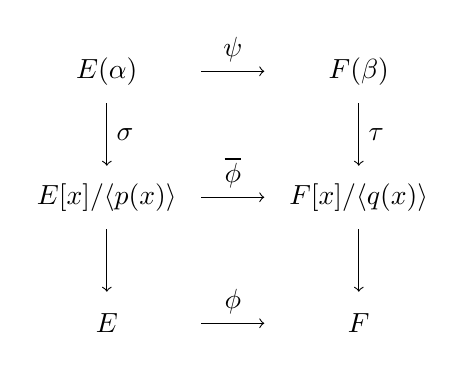
\begin{tikzpicture}[scale=0.8] %Replaced figure with tikz figure - TWJ 8/29/2010

\draw [<-] (0,0.5) -- (0,1.5);
\draw [<-] (0,2.5) -- (0,3.5);


\draw [<-] (4,0.5) -- (4,1.5);
\draw  [<-] (4,2.5) -- (4,3.5);


\draw [->] (1.5,0) -- (2.5,0);
\draw [->] (1.5,2) -- (2.5,2);
\draw [->] (1.5,4) -- (2.5,4);


\node at (0,0)  {$E$};
\node at (4,0)  {$F$};

\node at (0,2)  {$E[x] / \langle p(x) \rangle$};
\node at (4,2)  {$F[x]/\langle q(x) \rangle$};

\node at (0,4)  {$E(\alpha)$};
\node at (4,4)  {$F(\beta)$};

\node [above] at (2,0) {$\phi$};
\node [above] at (2,2) {$\overline{\phi}$};
\node [above] at (2,4) {$\psi$};

\node [right] at (0,3) {$\sigma$};
\node [right] at (4,3) {$\tau$};

\end{tikzpicture}
\end{center}

We leave the proof of uniqueness as a exercise.
\end{proof}

 
\begin{theorem}\label{fields:isomorph_extension_theorem}
Let $\phi : E \rightarrow F$ be an isomorphism of fields and let 
$p(x)$ be a nonconstant polynomial in $E[x]$ and $q(x)$
the corresponding polynomial in $F[x]$ under the isomorphism. If $K$ is
a splitting field of $p(x)$ and $L$ is a splitting field of $q(x)$,
then $\phi$ extends to an isomorphism $\psi : K \rightarrow L$.
\end{theorem}


\begin{proof}
We will use mathematical induction on the degree of $p(x)$. We can
assume that $p(x)$ is irreducible over $E$. Therefore, $q(x)$ is also
irreducible over $F$. If $\deg p(x) = 1$, then by the definition of a
splitting field, $K = E$ and $L = F$ and there is nothing to prove. 


Assume that the theorem holds for all polynomials of degree less than
$n$. Since $K$ is a splitting field of $E$, all of the roots of $p(x)$
are in $K$. Choose one of these roots, say $\alpha$, such that $E
\subset E( \alpha ) \subset K$. Similarly, we can find a root $\beta$
of $q(x)$ in $L$ such that $F \subset F( \beta) \subset L$. 
By Lemma~\ref{fields:isomorph_lemma}, there exists an isomorphism $\overline{\phi} : E(
\alpha ) \rightarrow F( \beta)$ such that $\overline{\phi}( \alpha ) =
\beta$  and $\overline{\phi}$ agrees with $\phi$ on $E$. 

\begin{center}
\tikzpreface{fields_splitting_isomorph}
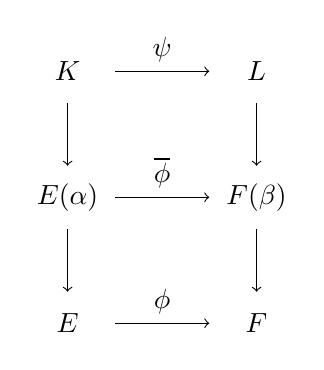
\begin{tikzpicture}[scale=0.8] %Replaced figure with tikz figure - TWJ 8/29/2010

\draw [<-] (0,0.5) -- (0,1.5);
\draw [<-] (0,2.5) -- (0,3.5);


\draw [<-] (3,0.5) -- (3,1.5);
\draw  [<-] (3,2.5) -- (3,3.5);


\draw [->] (0.75,0) -- (2.25,0);
\draw [->] (0.75,2) -- (2.25,2);
\draw [->] (0.75,4) -- (2.25,4);


\node at (0,0)  {$E$};
\node at (3,0)  {$F$};

\node at (0,2)  {$E( \alpha )$};
\node at (3,2)  {$F( \beta )$};

\node at (0,4)  {$K$};
\node at (3,4)  {$L$};

\node [above] at (1.5,0) {$\phi$};
\node [above] at (1.5,2) {$\overline{\phi}$};
\node [above] at (1.5,4) {$\psi$};



\end{tikzpicture}
\end{center}

Now write
$p(x) = (x - \alpha ) f(x)$ and $q(x) = ( x - \beta) g(x)$, where the
degrees of $f(x)$ and $g(x)$ are less than the degrees of $p(x)$ and
$q(x)$, respectively. The field extension $K$ is a splitting field for
$f(x)$ over $E( \alpha)$, and $L$ is a splitting field for $g(x)$
over $F( \beta )$. By our induction hypothesis there exists an
isomorphism  $\psi : K \rightarrow L$ such that $\psi$ agrees with
$\overline{\phi}$ on $E( \alpha)$. Hence, there exists an isomorphism
$\psi : K \rightarrow L$ such that $\psi$ agrees with $\phi$ on $E$. 
\end{proof}


\begin{corollary}\label{fields:splitting_field_corollary}
Let $p(x)$ be a polynomial in $F[x]$. Then there exists a splitting
field $K$ of $p(x)$ that is unique up to isomorphism. 
\end{corollary}


 
\section{Geometric Constructions}


In ancient Greece, three classic problems were posed. These problems
are geometric in nature and involve straightedge-and-compass
constructions from what is now high school geometry; that is, we are
allowed to use only a straightedge and compass to solve them. The
problems can be stated as follows.    
\begin{enumerate}

\item
Given an arbitrary angle, can one trisect the angle into three equal
subangles using only a straightedge and compass?

\item
Given an arbitrary circle, can one construct a square with the same
area using only a straightedge and compass?

\item
Given a cube, can one construct the edge of another cube having twice
the volume of the original? Again, we are only allowed to use a
straightedge and compass to do the construction.

\end{enumerate}
After puzzling mathematicians for over two thousand years, each of
these constructions was finally shown to be impossible.  We will use
the theory of fields to provide a proof that the solutions do not
exist.  It is quite remarkable that the long-sought solution to each
of these three geometric problems came from abstract algebra.  


First, let us determine more specifically what we mean by a
straightedge and compass, and also examine the nature of these
problems in a bit more depth.  To begin with, {\em a straightedge is
not a ruler}. We cannot measure arbitrary lengths with a straightedge.
It is merely a tool for drawing a line through two points. The
statement that the trisection of an arbitrary angle is impossible
means that there is at least one angle that is impossible to trisect
with a straightedge-and-compass construction. Certainly it is
possible to trisect an angle in special cases.  We can construct a
$30^\circ$ angle; hence, it is possible to trisect a $90^\circ$
angle.  However, we will show that it is impossible to construct a 
$20^\circ$ angle.  Therefore, we cannot trisect a $60^\circ$ angle. 

 

\subsection*{Constructible Numbers}
 

A real number $\alpha$ is {\bfi constructible\/}\index{Constructible
number} if we can construct a line segment of length $| \alpha |$ in a
finite number of steps from a segment of unit length by using a
straightedge and compass.  
 

\begin{theorem}\label{fields:construct_num_ther}
The set of all constructible real numbers forms a subfield $F$ of the
field of real numbers. 
\end{theorem}
 
 
\begin{proof}
Let $\alpha$ and $\beta$ be constructible numbers.  We must show that
$\alpha + \beta$, $\alpha - \beta$, $\alpha \beta$, and $\alpha /
\beta$ ($\beta \neq 0$) are also constructible numbers. We can assume
that both $\alpha$ and $\beta$ are positive with $\alpha > \beta$. It
is quite obvious how to construct $\alpha + \beta$ and $\alpha -
\beta$. To find a line segment with length $\alpha \beta$, we assume
that $\beta > 1$ and construct the triangle in Figure~\ref{Multiply}
such that triangles $\triangle ABC$ and $\triangle ADE$ are similar.
Since $\alpha / 1 = x / \beta$, the line segment $x$ has length
$\alpha \beta$.  A similar construction can be made if $\beta <1$. We
will leave it as an exercise to show that the same triangle can be
used to construct $\alpha / \beta$ for $\beta \neq 0$.  
\end{proof}

\begin{figure}[htb]
\begin{center}
\tikzpreface{fields_multiply}
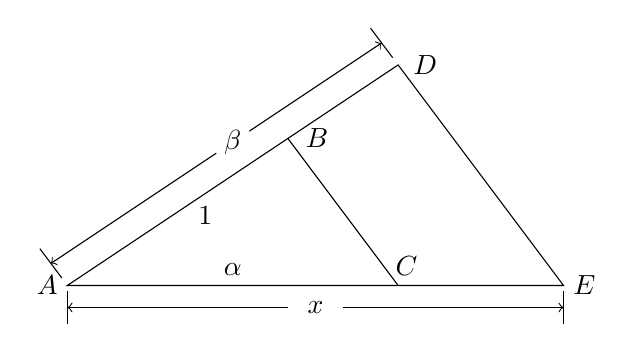
\begin{tikzpicture}[scale=0.7] %Replaced figure with tikz figure and corrected figure - TWJ 8/19/2010

\draw  (0,0) node [left] {$A$} -- (9,0) node [right] {$E$} -- (6,4) -- cycle;
\draw  (6,0)  -- (4,2.667);

\draw  (0,-0.1) -- (0,-0.7);
\draw  (9,-0.1) -- (9,-0.7);
\draw [<-] (0,-0.4) -- (4,-0.4);
\draw [->] (5,-0.4) -- (9,-0.4);

\draw (-0.1,0.133) -- (-0.5,0.667);
\draw (5.9,4.133) -- (5.5,4.667);
\draw [<-]  (-0.3, 0.4) -- (2.7,2.4);
\draw [->]  (3.3,2.8) -- (5.7,4.4);

\node [right] at (4.15,2.667)  {$B$};
\node [above] at (6.15,0)  {$C$};
\node [right] at (6.1,4)  {$D$};
\node [below] at (2.5,1.6)  {$1$};
\node [above] at (3,0)  {$\alpha$};
\node at (3,2.6)  {$\beta$};
\node at (4.5,-0.4)  {$x$};

\end{tikzpicture}

\end{center}
\caption{Construction of products}
\label{Multiply}
\end{figure}


\begin{lemma}
If $\alpha$ is a constructible number, then $\sqrt{\alpha}$ is a
constructible number.
\end{lemma}


\begin{proof}
In Figure~\ref{Root} the triangles $\triangle ABD$, $\triangle BCD$,
and $\triangle ABC$ are similar; hence, $1 /x = x / \alpha$, or $x^2 =
\alpha$. 
\end{proof}

\begin{figure}[htb]
\begin{center}
\tikzpreface{fields_root}
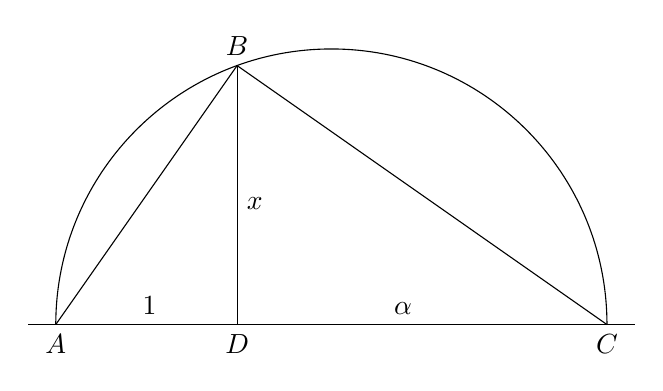
\begin{tikzpicture}[scale=0.7] %Replaced figure with tikz figure and corrected figure - TWJ 8/19/2010


\draw  (-5.5,0) -- (5.5,0);
\draw (5,0) arc (0:180:5);
\draw (5,0) -- (110:5) -- (-5,0);
\draw (110:5) -- (110:5 |- 0,0) node [below] {$D$};

\node [below] at (-5,0)  {$A$};
\node [below] at (5,0)  {$C$};
\node [above] at (110:5)  {$B$};
\node [above] at (1.3,0)  {$\alpha$};
\node [above] at (-3.3,0)  {1};
\node [right] at (110:5 |- 0,2.2) {$x$};

\end{tikzpicture}
\end{center}
\caption{Construction of roots}
\label{Root}
\end{figure}



\medskip


By Theorem~\ref{fields:construct_num_ther}, we can locate in the plane any point $P =( p, q)$
that has rational coordinates $p$ and $q$. We need to know what other
points can be constructed with a compass and straightedge from points
with rational coordinates.  


\begin{lemma}
Let $F$ be a subfield of ${\mathbb R}$.
\begin{enumerate}

\rm \item \it
If a line contains two points in $F$, then it has the equation $a x + by
+ c = 0$, where $a$, $b$, and $c$ are in $F$.

\rm \item \it
If a circle has a center at a point with coordinates in $F$ and a radius
that is also in $F$, then it has the equation $x^2 + y^2 + d x + e y
+ f = 0$, where $d$, $e$, and $f$ are in $F$.

\end{enumerate}
\end{lemma}


\begin{proof}
Let $(x_1, y_1)$ and $(x_2, y_2)$ be points on a line whose
coordinates are in $F$.  If $x_1 = x_2$, then the equation of the line
through the two points is $x - x_1 = 0$, which has the form $a x + by +
c = 0$.  If $x_1 \neq x_2$, then the equation of the line through the
two points is given by  
\[
y - y_1 = \left( \frac{y_2 - y_1}{x_2 - x_1} \right) (x - x_1),
\]
which can also be put into the proper form.


To prove the second part of the lemma, suppose that $(x_1, y_1)$ is the
center of a circle of radius $r$.  Then the circle has the equation
\[
(x - x_1)^2 + (y - y_1)^2 - r^2 = 0.
\]
This equation can easily be put into the appropriate form.
\end{proof}


\medskip


Starting with a field of constructible numbers $F$, we have three 
possible ways of constructing additional points in ${\mathbb R}$ with a
compass and straightedge. 
\begin{enumerate}
 
\item 
To find possible new points in ${\mathbb R}$, we can take the
intersection of two lines, each of which passes through two known
points with coordinates in $F$. 
 
\item 
The intersection of a line that passes through two points that have 
coordinates in $F$ and a circle whose center has coordinates in $F$ 
with radius of a length in $F$ will give new points in ${\mathbb R}$.
 
\item 
We can obtain new points in ${\mathbb R}$ by intersecting two
circles whose centers have coordinates in $F$ and whose radii are of
lengths in $F$.
 
\end{enumerate}
The first case gives no new points in ${\mathbb R}$, since the solution 
of two equations of the form $a x + by + c = 0$ having coefficients in
$F$ will always be in $F$. The third case can be reduced to the second
case.  Let
\begin{align*}
x^2 + y^2 + d_1 x +e_1 x + f_1 = 0 \\
x^2 + y^2 + d_2 x +e_2 x + f_2 = 0
\end{align*}
be the equations of two circles, where $d_i$, $e_i$, and $f_i$ are in
$F$ for $i = 1, 2$. These circles have the same intersection as the
circle  
\[
x^2 + y^2 + d_1 x +e_1 x + f_1 = 0 
\] and the line
\[
(d_1 - d_2) x + b(e_2 - e_1)y + (f_2 - f_1) = 0.
\]
The last equation is that of the chord passing through the
intersection points of the two circles. Hence, the intersection of two
circles can be reduced to the case of an intersection of a line with a
circle. 
 

Considering the case of the intersection of a line and a circle, we
must determine the nature of the solutions of the equations
\begin{align*}
a x + by + c & = 0 \\
x^2 + y^2 + d x + e y + f & = 0.
\end{align*}
If we eliminate $y$ from these equations, we obtain an equation of
the form $Ax^2 + B x + C = 0$, where $A$, $B$, and $C$ are in $F$. The
$x$ coordinate of the intersection points is given by
\[
x = \frac{- B \pm \sqrt{B^2 - 4 A C} }{2 A}
\]
and is in $F( \sqrt{\alpha}\, )$, where $\alpha = B^2 - 4 A C > 0$.
We have proven the following lemma.

 
\begin{lemma}\label{fields:lines_and_circles_lemma}
Let $F$ be a field of constructible numbers. Then the points
determined by the intersections of lines and circles in $F$ lie in the
field $F( \sqrt{\alpha}\, )$ for some $\alpha$ in $F$.  
\end{lemma}
 
 
\begin{theorem}
A real number $\alpha$ is a constructible number if and only if there
exists a  sequence of fields
\[
{\mathbb Q} = F_0 \subset F_1 \subset \cdots \subset F_k
\]
such that $F_i = F_{i-1}( \sqrt{ \alpha_i}\, )$ with $\alpha_i \in F_i$ 
and  $\alpha \in F_k$. 
In particular, there exists an integer $k > 0$ such that 
$[{\mathbb Q}(\alpha) : {\mathbb Q} ] = 2^k$.
\end{theorem} %Clarified where $\alpha_i$ lives - TWJ 4/23/2011
 
 
\begin{proof}
The existence of the $F_i$'s and the $\alpha_i$'s is a direct
consequence of Lemma~\ref{fields:lines_and_circles_lemma} and of the fact that
\[
[F_k: {\mathbb Q}] = [F_k : F_{k-1}][F_{k-1} : F_{k-2}] \cdots [F_1:
{\mathbb Q} ] = 2^k.
\]
\end{proof}


\begin{corollary}
The field of all constructible numbers is an algebraic extension of
${\mathbb Q}$.
\end{corollary}
 

As we can see by the field of constructible numbers, not every
algebraic extension of a field is a finite extension. 
 


\subsection*{Doubling the Cube and Squaring the Circle}
 

We are now ready to investigate the classical problems of doubling
the cube and squaring the circle.  We can use the field of
constructible numbers to show exactly when a particular geometric
construction can be accomplished.    

 
{\em Doubling the cube is impossible\index{Doubling the cube}}.  Given the
edge of the cube, it is impossible to construct with a straightedge
and compass the edge of the cube that has twice the volume of the
original cube. Let the original cube have an edge of length 1 and,
therefore, a volume of  1. If we could construct a cube having a
volume of 2, then this new cube would have an edge of length
$\sqrt[3]{2}$. However, $\sqrt[3]{2}$ is a zero of the irreducible
polynomial $x^3 -2$ over ${\mathbb Q}$; hence, 
\[
[{\mathbb Q}(\sqrt[3]{2}\, ) : {\mathbb Q}] =3
\]
This is impossible, since 3 is not a power of 2.
 
 
{\em Squaring the circle\index{Squaring the circle} is impossible}.
Suppose that we have a circle of radius 1.  The area of the circle 
is $\pi$; therefore, we must be able to construct a square with side
$\sqrt{\pi}$. This is impossible since $\pi$ and consequently
$\sqrt{\pi}$ are both transcendental. Therefore, using a straightedge
and compass, it is not possible to construct a square with the same
area as the circle.  
 


\subsection*{Trisecting an Angle}\index{Trisection of an angle}
 

{\em Trisecting an arbitrary angle is impossible}.  We will show that
it is impossible to construct a $20^\circ$ angle.  Consequently, a
$60^{\circ}$ angle cannot be trisected. We first need to calculate
the triple-angle formula for the cosine: 
\begin{align*}
\cos 3 \theta & = \cos( 2 \theta + \theta ) \\
& =
\cos 2 \theta \cos \theta - \sin 2 \theta \sin \theta \\
& =
( 2 \cos^2 \theta - 1) \cos \theta - 2 \sin^2 \theta \cos
\theta \\
& =
( 2 \cos^2 \theta - 1) \cos \theta - 2 (1- \cos^2 \theta)
\cos \theta \\
& =
4 \cos^3 \theta - 3 \cos \theta.
\end{align*}
The angle $\theta$ can be constructed if and only if $\alpha = \cos
\theta$ is constructible. Let $\theta = 20^{\circ}$. Then $\cos 3
\theta =  \cos 60^\circ = 1/2$. By the triple-angle formula for the
cosine,
\[
4 \alpha^3 - 3 \alpha = \frac{1}{2}.
\]
Therefore, $\alpha$ is a zero of $8 x^3 - 6 x -1$.  This polynomial
has no factors in ${\mathbb Z}[x]$, and hence is irreducible over ${\mathbb
Q}[x]$. Thus, $[{\mathbb Q}( \alpha ) : {\mathbb Q }] = 3$. Consequently,
$\alpha$ cannot be a constructible number.
 
 

\histhead


\noindent{\small \histf
Algebraic number theory uses the tools of algebra to solve problems in
number theory.  Modern algebraic number theory began with
Pierre de Fermat\index{Fermat, Pierre de} (1601--1665). Certainly we
can find many positive integers that satisfy the equation $x^2 + y^2 =
z^2$; Fermat conjectured that the equation $x^n + y^n = z^n$ has no
positive integer solutions for $n \geq 3$.  He stated in the margin of
his copy of the Latin translation of Diophantus' {\it Arithmetica}
that he had found a marvelous proof of this theorem, but that the
margin of the book was too narrow to contain it.    Building on work of other mathematicians, it was Andrew Wiles who finally succeeded in proving Fermat's Last Theorem in the 1990s. Wiles's achievement was reported on the front page of the {\it New York Times}.


Attempts to prove Fermat's Last Theorem have led to important
contributions to algebraic number theory by such notable
mathematicians as Leonhard Euler\index{Euler, Leonhard} (1707--1783).
Significant advances in the understanding of Fermat's Last
Theorem were made by Ernst Kummer\index{Kummer, Ernst} (1810--1893). 
Kummer's student, Leopold \mbox{Kronecker}\index{Kronecker, Leopold}
(1823--1891), became one of the leading algebraists of the nineteenth
century. \mbox{Kronecker's} theory of  ideals and his study of algebraic
number theory added much to the understanding of fields. 


David Hilbert\index{Hilbert, David} (1862--1943) and Hermann
Minkowski\index{Minkowski, Hermann} (1864--1909) were
among the mathematicians who led the way in this subject at the  
beginning of the twentieth century.  Hilbert and Minkowski were both
mathematicians at G\"{o}ttingen University in Germany. G\"{o}ttingen
was truly one the most important centers of mathematical research
during the last two centuries. The large number of exceptional
mathematicians who studied there included Gauss, Dirichlet, Riemann,
Dedekind, Noether, and~Weyl.


Andr\'{e} Weil\index{Weil, Andr\'{e}} answered questions in number theory
using algebraic geometry, a field of mathematics that studies geometry
by studying commutative rings. From about 1955 to 1970, A.
Grothendieck\index{Grothendieck, A.} dominated the field of algebraic
geometry. Pierre Deligne\index{Deligne, Pierre}, a student of
Grothendieck, solved several of Weil's number-theoretic conjectures.
One of the most recent contributions to algebra and number theory is
Gerd Falting's\index{Faltings, Gerd} proof of the Mordell-Weil
conjecture\index{Mordell-Weil conjecture}. This conjecture of
Mordell and Weil essentially says that certain polynomials $p(x, y )$ in
${\mathbb Z}[x,y]$ have only a finite number of integral solutions.  
\histbox
} 


 
\markright{EXERCISES}
\section*{Exercises}
\exrule

 
{\small
\begin{enumerate}


\item
Show that each of the following numbers is algebraic over ${\mathbb Q}$
by finding the minimal polynomial of the number over ${\mathbb Q}$.
\begin{enumerate}

 \item
$\sqrt{ 1/3 + \sqrt{7} }$

 \item
$\sqrt{ 3} + \sqrt[3]{5}$

 \item
$\sqrt{3} + \sqrt{2}\, i$

 \item
$\cos \theta + i \sin \theta$ for $\theta = 2 \pi /n$ with $n \in
{\mathbb N}$

 \item
$\sqrt{ \sqrt[3]{2} - i }$

\end{enumerate}


\item
Find a basis for each of the following field extensions. What is the
degree of each extension?
\begin{enumerate}
 
 \item
${\mathbb Q}( \sqrt{3}, \sqrt{6}\, )$ over ${\mathbb Q}$
 
 \item
${\mathbb Q}( \sqrt[3]{2}, \sqrt[3]{3}\, )$ over ${\mathbb Q}$

 \item
${\mathbb Q}( \sqrt{2}, i)$ over ${\mathbb Q}$

 \item
${\mathbb Q}( \sqrt{3}, \sqrt{5}, \sqrt{7}\, )$ over ${\mathbb Q}$
 
 \item
${\mathbb Q}( \sqrt{2}, \root 3 \of{2}\, )$ over ${\mathbb Q}$

 \item
${\mathbb Q}( \sqrt{8}\, )$ over ${\mathbb Q}(\sqrt{2}\, )$ 

 \item
${\mathbb Q}(i, \sqrt{2} +i, \sqrt{3} + i )$ over ${\mathbb Q}$

 \item
${\mathbb Q}( \sqrt{2} + \sqrt{5}\, )$ over ${\mathbb Q} ( \sqrt{5}\, )$

 \item
${\mathbb Q}( \sqrt{2}, \sqrt{6} + \sqrt{10}\, )$ over ${\mathbb Q} ( \sqrt{3}
+ \sqrt{5}\, )$

\end{enumerate}



\item
Find the splitting field for each of the following polynomials.
\begin{multicols}{2}
\begin{enumerate}

\item
$x^4 - 10 x^2 + 21$ over ${\mathbb Q}$

\item
$x^4 + 1$ over ${\mathbb Q}$

\item
$x^3 + 2x + 2$ over ${\mathbb Z}_3$

\item
$x^3 - 3$ over ${\mathbb Q}$


\end{enumerate}
\end{multicols}


\item
Determine all of the subfields of ${\mathbb Q}( \sqrt[4]{3}, i )$.

 
\item
Show that ${\mathbb Z}_2[x] / \langle x^3 + x + 1 \rangle$ is a field
with eight elements. Construct a multiplication table for the
multiplicative group of the field. 


\item
Show that the regular 9-gon is not constructible with a straightedge
and compass, but that the regular 20-gon is constructible.  
 

\item
Prove that the cosine of one degree ($\cos 1^\circ$) is algebraic over
${\mathbb Q}$ but not constructible.


\item
Can a cube be constructed with three times the volume of a given cube?


%***********************************THEORY***************************


\item
Prove that ${\mathbb Q}(\sqrt{3}, \sqrt[4]{3}, \sqrt[8]{3}, \ldots )$ 
is an algebraic extension of ${\mathbb Q}$ but not a finite extension. 


\item
Prove or disprove: $\pi$ is algebraic over ${\mathbb Q}(\pi^3)$.


\item
Let $p(x)$ be a nonconstant polynomial of degree $n$ in $F[x]$.  Prove
that there exists a splitting field $E$ for $p(x)$ such that $[E : F]
\leq n!$. 


\item
Prove or disprove: ${\mathbb Q}( \sqrt{2}\, ) \cong {\mathbb Q}( \sqrt{3}\, )$.


\item
Prove that the fields ${\mathbb Q}(\sqrt[4]{3}\, )$ and ${\mathbb
Q}(\sqrt[4]{3}\, i)$ are isomorphic but not equal.


\item
Let $K$ be an algebraic extension of $E$, and $E$ an algebraic
extension of $F$. Prove that $K$ is algebraic over $F$. [{\em
Caution}: Do not assume that the extensions are finite.]


\item
Prove or disprove: ${\mathbb Z}[x] / \langle x^3 -2 \rangle$ is a field.


\item
Let $F$ be a field of characteristic $p$. Prove that $p(x) = x^p - a$
either is irreducible over $F$ or splits in $F$. 


\item
Let $E$ be the algebraic closure of a field $F$. Prove that every
polynomial $p(x)$ in $F[x]$ splits in $E$.


\item
If every irreducible polynomial $p(x)$ in $F[x]$ is linear, show that
$F$ is an algebraically closed field.


\item
Prove that if $\alpha$ and $\beta$ are constructible numbers such that
$\beta \neq 0$, then so is $\alpha / \beta$. 


\item
Show that the set of all elements in ${\mathbb R}$ that are algebraic 
over ${\mathbb Q}$ form a field extension of ${\mathbb Q}$ that is not
finite. 

 
\item
Let $E$ be an algebraic extension of a field $F$, and let $\sigma$ be
an automorphism of $E$ leaving $F$ fixed. Let $\alpha \in E$. Show
that $\sigma$ induces a permutation of the set of all zeros of the
minimal polynomial of $\alpha$ that are in $E$. 

 
\item
Show that ${\mathbb Q}( \sqrt{3}, \sqrt{7}\, ) = {\mathbb Q}( \sqrt{3} +
\sqrt{7}\, )$.  Extend your proof to show that ${\mathbb Q}( \sqrt{a},
\sqrt{b}\, ) = {\mathbb Q}( \sqrt{a} + \sqrt{b}\, )$. 
 

\item
Let $E$ be a finite extension of a field $F$. If $[E:F]=2$, show that
$E$ is a splitting field of $F$.


\item
Prove or disprove: Given a polynomial $p(x)$ in ${\mathbb Z}_6[x]$, it is
possible to construct a ring $R$ such that $p(x)$ has a root in
$R$. 


\item
Let $E$ be a field extension of $F$ and $\alpha \in E$.  Determine
$[F(\alpha): F(\alpha^3)]$.


\item
Let $\alpha, \beta$ be transcendental over ${\mathbb Q}$. Prove that
either $\alpha \beta$ or $\alpha + \beta$ is also transcendental.


\item
Let $E$ be an extension field of $F$ and $\alpha \in E$ be
transcendental over $F$.  Prove that every element in $F(\alpha)$
that is not in $F$ is also transcendental over $F$.


\end{enumerate}
}
 
 
 
 
\subsection*{References and Suggested Readings}
 
{\small
\begin{itemize}



 
\item[{\bf [1]}] %Out of print  - 19 August 2010 - TWJ
Dean, R. A. {\it Elements of Abstract Algebra}. Wiley, New
York, 1966.

\item[{\bf [2]}] %Out of print  - 19 August 2010 - TWJ
Dudley, U. {\it A Budget of Trisections}. Springer-Verlag, New
York, 1987. An interesting and entertaining account of how not to 
trisect an angle.

\item[{ \bf [3]}] %Reference updated - 19 August 2010 - TWJ
Fraleigh, J. B. 
{\it A First Course in Abstract Algebra}. 7th ed.
Pearson, Upper Saddle River, NJ, 2003. 
 
\item[{\bf [4]}] %Out of print  - 19 August 2010 - TWJ
Kaplansky, I. {\it Fields and Rings}, 2nd ed. University of Chicago
Press, Chicago, 1972. 
 
\item[{\bf [5]}] %This book is available through Nabu Press, a print on demand publisher that sells through Amazon  - 19 August 2010 - TWJ
Klein, F. {\it Famous Problems of Elementary Geometry}.
Chelsea, New York, 1955.

\item[{\bf [6]}] %Reference added - 19 August 2010 - TWJ
Martin, G.
{\it Geometric Constructions}.
Springer, New York, 1998.

\item[{\bf [7]}] %Reference updated - 19 August 2010 - TWJ
H. Pollard and H. G. Diamond. {\it  Theory of Algebraic Numbers},
Dover, Mineola, NY, 2010.

\item[{\bf [8]}] %Out of print  - 19 August 2010 - TWJ
Walker, E. A. {\it Introduction to Abstract Algebra}. Random House, 
New York, 1987. This work contains a proof showing that every 
field has an algebraic closure.
 
\end{itemize}
}





